%!TEX root = ../report.tex

% 
% Overview
% 

\section{Overview} % (fold)
\label{sec:overview}


This Section will provide an overview over this topic providing background (\dots). The Section~\ref{sec:objectives} will address the objectives for this thesis work. Section~\ref{sec:related_work} will explore different related works to this program. Section~\ref{sec:architecture} will describe the architecture of the proposed solution. Section~\ref{sec:evaluation} will explain how our results will be evaluated and we will conclude on Section~\ref{sec:conclusions}.

\subsection{Procedural Generation} % (fold)
\label{sub:procedural_generation}


Procedural Generation is the algorithmic generation of content in stead of the usual manual creation of content. This can be applied in almost all forms of content, but is mostly used in graphics creation and sound (music and synthetic speech).

The key property of procedural generation is that in describes the data entity, be it geometry, texture or effect, in terms of a sequence of generation instructions rather than as a static block of data \cite{Kelly}. This allows anyone with less resources to produce high detailed, and high quality content.

%!TEX root = ../report.tex

\subsection{Procedural Modelling Techniques} % (fold)
\label{sub:procedural_modelling_techniques}

\subsubsection{Fractals} % (fold)
\label{ssub:fractals}


A fractal is a never-ending pattern. Fractals are infinitely complex patterns that are self-similar across different scales. 
This concept is observed in some forms that exist in nature. From trees, mountains, coastlines to the network of neurons on a human cortex can be seen as examples of fractals. Natural shapes tend to be irregular and fragmented and exhibit a complexity incomparable to regular geometry [Mandelbrot 1982]. The Figure~\ref{fig:NFractals} shows some examples of that. 



\begin{figure}
        \centering
        \begin{subfigure}[b]{0.4\textwidth}
                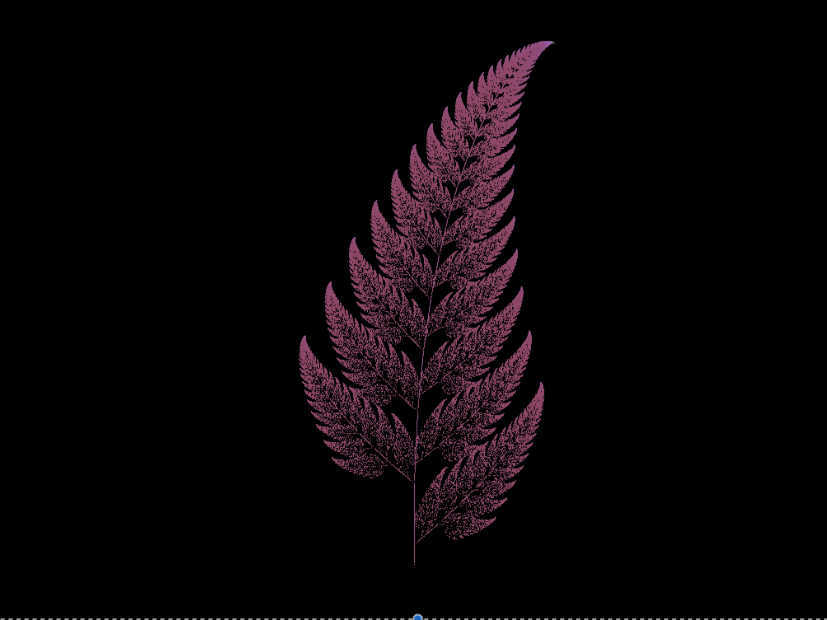
\includegraphics[width=\textwidth]{img/Theory/Fractals/Leaf.png}
                
                \label{fig:gull}
        \end{subfigure}%
        ~ %add desired spacing between images, e. g. ~, \quad, \qquad, \hfill etc.
          %(or a blank line to force the subfigure onto a new line)
        \begin{subfigure}[b]{0.4\textwidth}
                
\includegraphics[width=\textwidth]{img/Theory/Fractals/Fractal_Broccoli.jpg}
                
                \label{fig:tiger}
        \end{subfigure}
        \caption{Fractals in Nature}\label{fig:NFractals}
\end{figure}




This idea was applied in maths with the evolution of a new area in this science called fractal mathematics. The objective of this field is to describe this very complex shapes. With really simple rules as repeating a substitution pattern. 

\begin{figure}[htbp]
	\centering
	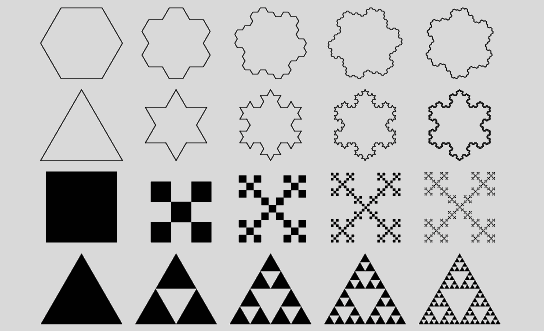
\includegraphics[width=0.9\textwidth]{img/Theory/Fractals/Fractal1_1000.png}
	\caption{Geometric Fractals}
	\label{fig:GFractals}
\end{figure}

In the Figure~\ref{fig:GFractals} there are four examples of Geometric Fractals, with the first five iterations of each one. All of them are built by the substitution of a part of the image by another one. 

The example of the second row is known as the Koch snowflake. In this example, at each iteration, all the line segments are replaced by four segments with 1/3 of the size of the original one with the two in the middle being placed in a angle forming a equilateral triangle with the original line that is removed.

It's clear that the detail that is presented in each iteration increases as the scale changes. To try to mesure this evolution there is the idea of ​​fractal dimension in which the detail in a pattern changes in comparison with the scale in which it is measured (Fractal\_dimension). 

A fractal shape is defined by a recursive algorithm and successive recursions create more detail. There is no theoretic limit to the recursion size and with this a fractal is infinitely detailed. 


% subsubsection fractals (end)



\subsubsection{Cellular Automaton} % (fold)
\label{ssub:cellular_automaton}


It's a model of a system of cells within a grid with a determined shape, each of this cells can be on one of a finite set of states. It evolves during a finite amount of time steps with a set of simple rules according with the state of the neighbouring cells.
The neighbourhood of the cell can be defined in many different ways, the most common is the use of the adjacent cells.

Starting from a line with zeros except the middle cell with one and the following set of rules:

\begin{figure}[htbp]
	\centering
	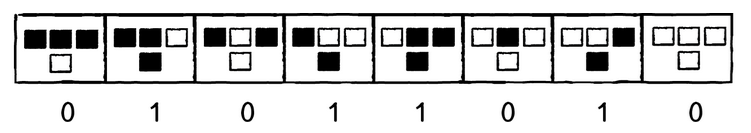
\includegraphics[width=0.85\textwidth]{img/Theory/Cellular_A/Rules.png}
	\caption{Example Production Rules\cite{Shiffman2012}}
	\label{fig:label}
\end{figure}



The Figure~\ref{fig:resultCA} image represents the evolution of one Cellular automaton over time.  In this case, each cell can have one of two states, black or white. Starting from a white line except the middle cell that is black and the presented set of rules.

\begin{figure}[htbp]
    \centering
    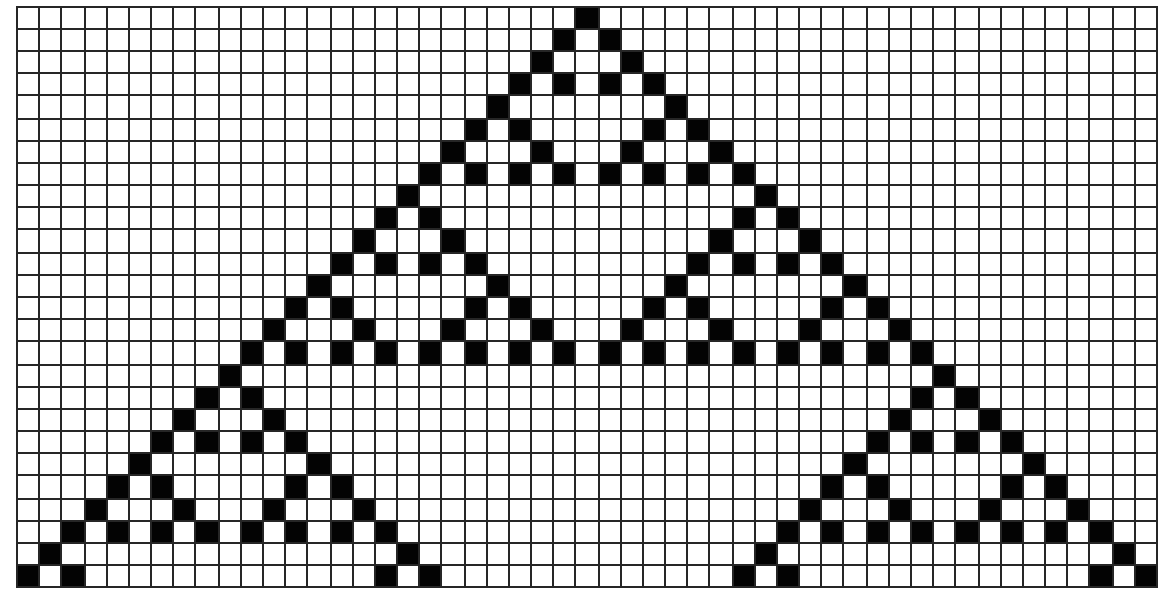
\includegraphics[width=0.85\textwidth]{img/Theory/Cellular_A/Result.png}
    \caption{caption}
    \label{fig:resultCA}
\end{figure}



Each line represents an iteration of the system with the application of the rules. With this set of rules Sierpiński triangle can be reproduced. 



L-Systems
Lindenmayer Systems (L-Systems) are a class of string rewriting mechanisms, originally developed by Lindenmayer as a mathematical theory of plant development.

One Lindenmayer-System, or L-System, is a type of a formal grammar and a string rewriting system that is capable of describe the behaviour of plant cells and model the growth processes of plant development.

It consists of two different parts, one axiom and a set of production rules. The axiom is the starting point of the system, acting as a seed. Then is't applied in this seed the set of production rules, that change the initial string and producing other strings.
This is an iterative process, so after the production of a larger set of strings, the rules can be applied to each one of them wish grows the size of the set even larger.

This L-Systems are used to produce natural growth of vegetation, and the generation of Fractals. 



All the Fractals in the image were generated using L-Systems. 
image from Wolfram MathWorld

In this process, each symbol is associated with a production rule. For instance having $\{a, b\}$ as our alphabet and $\{a=>ab, b=> bab\}$. From a starting axiom \emph{aba}, and the application of the rules we have:\\
\\
\centerline{a b a}
\centerline{ab bab ab}
\centerline{ab bab bab ab bab ab bab}
\centerline{ab bab bab ab bab bab ab bab ab bab bab ab bab ab bab bab ab bab}
\\
\\
This is an example of the evolution of one system. Note that the space between the symbols are just for readability.

% subsubsection cellular_automaton (end)

\subsubsection{Shape Grammars} % (fold)
\label{ssub:shape_grammars}


Shape Grammars can be considered grammars for design. In stead of having symbols or letters as components of the alphabet, they have shapes that can by in 2D or 3D. So the rules are constructed with this shapes, and specify the evolution of the system. With this process, similar to the L-Systems explained before, the shape starts small and simple and can evolve to one big and/or complex shape.

The process is performed in two steps, the recognition of a shape and the replacement according to the rules that are previously defined. 

The following images exemplify one shape grammar, with one rule and the evolution of the application of this rule to the shapes iteratively.



In this image, it's shown that from very simple initial shape, can be generated a complex from with a few iterations.




This is applied to the generation of buildings in the CityEngine system, using 3D blocks.





The figure on the right shows a simple building that I modelled using CityEngine and it's CGA Shape Grammar. But CGA is powerful enough to model much more complex buildings like the one at the bottom.

 













% subsubsection shape_grammars (end)




\subsubsection{Noise} % (fold)
\label{ssub:noise}


"To generate irregular procedural textures, we need an irregular primitive function,
usually called noise." It's a pseudorandom function that gave the goal to break the monotony of a pattern and make it look more random.
Perlin Noise is the most known and used noise function. It was created by Ken Perlin, for the movie Tron 1982 with the aiming to generate natural looking textures.
With this pseudorandom function, it's generated a sequence of values that are interpolated to generate a coherent noise. With the composition of several layers of this noise it's build a texture that look natural and with fractal like structure.




 For instance, the image above shows the result of six noise functions with different frequencies and amplitudes. And the sum of all this functions is the following.

``You may even imagine that it looks a little like a mountain range."

Source: \url{http://freespace.virgin.net/hugo.elias/models/m_perlin.htm}



% subsubsection noise (end)


\subsubsection{Tiling} % (fold)
\label{ssub:tiling}

A common solution to give realism to 3D objects is the application of textures. One problem is that this textures takes a lot of memory. To work around this problem an easy solution is to have a small texture piece, a tile, and repeat throughout the objects. And this is called tiling. Or as defined in Wolfram: ``A plane-filling arrangement of plane figures or its generalisation to higher dimensions.".  This means, the result constructing a plane from a finite set of ``tiles". 
If this technique is use naively commonly results in not very homogeneous textures, it depends much on the set of tiles that are used. If the borders of all the tiles are the same the result is always homogeneous. But if the borders are very different the chances to have a not uniform texture rises. This example from \cite{ProcWorld} shows how a bad structured tiling system produces a not homogeneous texture.  





To make uniform planes, the boundary of each tile must be coherent, i. e., the borders of connecting tiles have to match. Given a single tile, the so-called first corona is the set of all tiles that have a common boundary point with the tile (including the original tile itself). From that, the simple method to create a homogeneous texture is to connect each tile with one that belongs to it's first corona.
The easy, most simple solution is to make sure that all the tiles have the same borders all around. With this property it's guaranteed that any created texture will be homogeneous. But this solution doesn't provide much irregularity and the results present repeating patterns. 


Wang Tiles is a solution named after Mr Hao Wang, that predicted that tiling was not possible. This process allows tiling with an arbitrary number of different vertical and horizontal borders and from that calculate the set of tiles that are needed to create a full texture without inconsistencies. 



As you might have noticed, the inner content of the tiles are not a problem. As we are trying to create the uniform textures by arranging this smaller pieces only the borders matter, so we can create a set of tiles with the same borders and whatever inner content we want. With this technique the result can be much more irregular. 



Corner Tiles \cite{LD06AWTCECC}:
One alternative to Wang tiles with the points to be coloured.
The vanilla wang tiles have problems in the diagonals that are not taken into account. They are the confrontation between four tiles which leads to less homogeneous texture if we the borders don't match. By using the corners, the problem goes to the sides, that despite being larger, are only the confrontation between two tiles and therefore it leads to a more homogeneous texture.

Genetic tile generation:
“The bottom line for me is, Wang tiles are amazing things until you try to use them seriously. They work great for stuff you can synthesise from the ground up. If you are trying to mix samples from real life, get ready for some trouble.”
\url{http://procworld.blogspot.pt/2013/01/tile-genetics.html}


% subsubsection tiling (end)


 \subsubsection{Voxels} % (fold)
 \label{ssub:voxels}
 Voxels

``Voxel is a combination of ``volume" and ``pixel" ". i. e. the equivalent to pixels in 3D. In other words, if a pixel is a tiny square that represents a part of an model in a plane (picture), a voxel is a cube that represents a part of a model in a space.
Because we usually want to model the world, or parts of it, that have three dimensions, it's easier to visualize this models with voxels.

(\dots?)
% subsubsection voxels (end)

% subsection procedural_modelling_techniques (end)



\subsection{Architectural Styles} % (fold)
\label{sub:architectural_styles}

Most buildings or other man made structures are classified by it's \emph{Architectural Style}. An architectural style is characterized by the features that make a building notable and historically identifiable. This style characterisics are related to form, building materials, construction methods, etc. and change trough different places and over the years. 

Even with this constant change in the styles there are some rules that we have to followed. The most obvious one is the chronological time.
If we are modelling a city from the 16th century it's wrong if we add buildings with styles form the 19th century. And we have to think also in a simmilar way with the places, if it's an asian city we do not add buildings with a known european layout.

And this correctness in relation to the architectural styles is also an important concern to this work.

% subsection architectural_styles (end)

% subsection procedural_generation (end)

% section overview (end)